% Created 2016-08-17 Wed 14:38
\documentclass[tikz]{standalone}

\usepackage[utf8]{inputenc}
\usepackage[T1]{fontenc}
\usepackage{helvet}
\usepackage{../../templates/msc}

\renewcommand{\familydefault}{\sfdefault}

\tikzset{
every picture/.style={
line width=1pt
}}

\usepackage{tikz}
\author{Holger Karl}
\date{\today}
\title{}


\usetikzlibrary{chains,shapes.multipart}
\usetikzlibrary{shapes,calc}
\usetikzlibrary{automata,positioning}

\tikzset{
queue/.pic={
  \draw[line width=1pt]
    (0,0) -- ++(2.75cm,0) -- ++(0,-1cm) -- ++(-2.75cm,0);
   \fill [fill=red!10] (2.75cm-#1*10pt, -1cm) -- (2.75cm-#1*10pt, 0) -- (2.75cm,0) -- (2.75cm,-1cm)-- cycle ;
   \foreach \Val in {1,...,#1}
     \draw  ([xshift=-\Val*10pt]2.75cm,0) -- ++(0,-1cm); 
  }}

\begin{document}
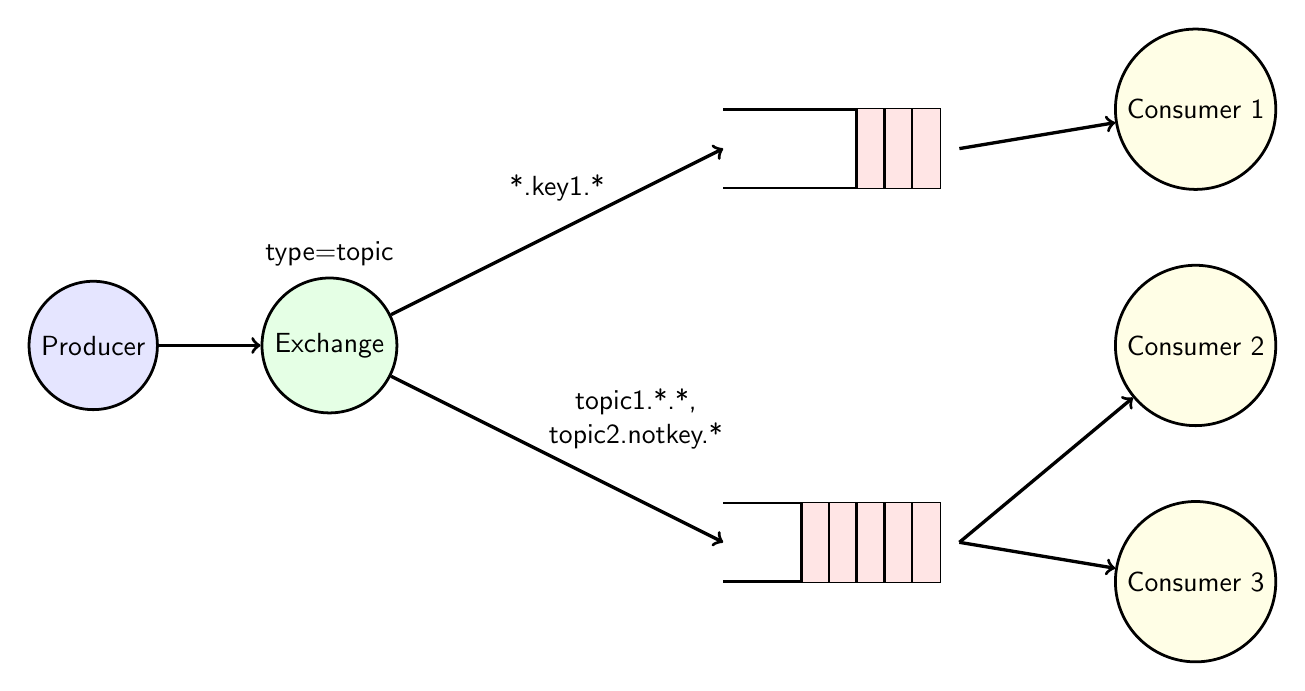
\begin{tikzpicture}[auto, 
block/.style = {rectangle, draw=black, thick, align=left}]

\node [draw,circle, fill=blue!10] at (0,0) (p) {Producer}; 
\node [draw,circle, fill=green!10] at (3,0) (e) {Exchange}; 
\node [above=of e,yshift=-1cm] {type=topic}; 

\path (8,3) pic  {queue=3}; 
\path (8,-2) pic  {queue=5}; 

\node [draw,circle, fill=yellow!10] at (14,-3) (c3) {Consumer 3}; 
\node [draw,circle, fill=yellow!10] at (14,0) (c2) {Consumer 2}; 
\node [draw,circle, fill=yellow!10] at (14,3) (c1) {Consumer 1}; 

\draw[->, very thick] (p) -- (e); 
\draw[->, very thick] (e) -- (8,2.5)  node [yshift=.25cm, above,midway] {*.key1.*}; 
\draw[->, very thick] (e) -- (8,-2.5) node [xshift=1cm, above,midway,align=center] {topic1.*.*,\\ topic2.notkey.*}; 

\draw[->, very thick] (11,-2.5) -- (c3); 
\draw[->, very thick] (11,-2.5) -- (c2); 
\draw[->, very thick] (11,2.5) -- (c1); 


\end{tikzpicture}
\end{document}